\section{Desarrollo y resultados}

A continuación, se detalla todo el desarrollo de la experiencia exponiendo como se hizo cada parte del enunciado. Cabe destacar que el desarrollo fue realizado en un sistema operativo Linux en base Debian, en específico se utilizó \textbf{elementary OS}.

\subsection{Capa física y de enlace}
Primeramente, se ha realizado un análisis de la red local, pasando desde los dispositivos que están conectados a la red, hasta porque medios lo están, pero primero se debe conocer las características asociadas a la red y las del mismo dispositivo donde se están ejecutando las pruebas. Entonces con la herramienta \verb|ifconfig| se puede saber cuál es la ip local del dispositivo además de un rango de ip de la red:

\begin{figure}[!ht]
	\centering
	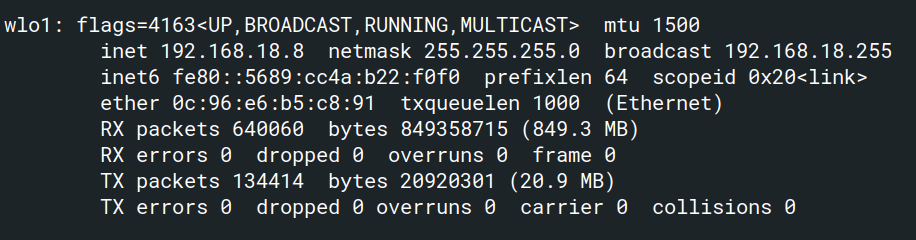
\includegraphics[scale=0.5]{images/ifconfig.png}
	\caption{Resultado de la ejecución de ifconfig}
	\label{if}
\end{figure}

\noindent Como se puede ver la figura \ref{if}, el dispositivo tiene la ip local \verb|192.168.18.8| además de que la red tiene un rango de ip de \verb|192.168.18.0| a \verb|192.168.18.255|.
\noindent Ahora para obtener información del adaptador de red del dispositivo se puede utilizar el siguiente comando:

\begin{lstlisting}
$ sudo lspci -nn | grep -i network
\end{lstlisting}

\begin{figure}[!ht]
	\centering
	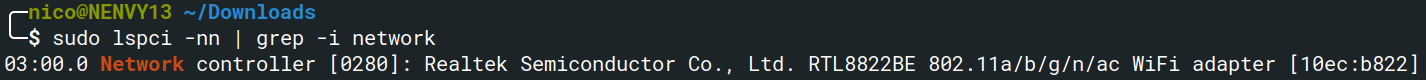
\includegraphics[scale=0.3]{images/lscpi.png}
	\caption{Resultado del comando lspci con información del adaptador de red}
	\label{lspci}
\end{figure}


\noindent Conociendo el dispositivo actual y el rango de ips local de la red se puede utilizar la herramienta \verb|nmap| para hacer un análisis de los dispositivos conectados a la red con sus ips y direcciones mac. Entonces si se ejecuta el siguiente comando: 

\begin{lstlisting}
$ sudo nmap -sn 192.168.18.1-255
\end{lstlisting}

\noindent Se obtiene la siguiente tabla de dispositivos:


\begin{table}[!h]
\begin{tabular}{|l|l|l|l|}
\hline
\textbf{Nombre de dispositivo} & \textbf{Capa física}  & \textbf{Dirección MAC} & \textbf{Dirección IP} \\ \hline
\_gateway(router)                 & \begin{tabular}[c]{@{}l@{}}Ethernet (802.3a) \\ WiFi 802.11a/b/g/n/ac\end{tabular}           & 24:a5:2c:4d:b4:17      & 192.168.18.1          \\ \hline
PC-Escritorio                  & Ethernet (802.3a)             & f0:79:59:92:b6:77      & 192.168.18.5          \\ \hline
Google-Home-Mini               & WiFi 802.11b/g/n/ac   & b0:2a:43:2d:86:84      & 192.168.18.6          \\ \hline
Desconocido                    & Wifi 802.11ac           & cc:9f:7a:3d:71:4c      & 192.168.18.7          \\ \hline
NENVY13                        & WiFi 802.11a/b/g/n/ac & 0c:96:e6:b5:c8:91      & 192.168.18.8          \\ \hline
HUAWEI\_Mate\_20\_l            & WiFi 802.11b/g/n/ac           & 88:bf:e4:21:12:b0      & 192.168.18.11         \\ \hline
Mi9T-MiTel?fono                & WiFi 802.11a/b/g/n/ac & a8:9c:ed:67:09:79      & 192.168.18.18         \\ \hline
Nintendo 3DS                   & WiFi 802.11b/g/n/ac   & 7c:bb:8a:64:b2:3b      & 192.168.18.19         \\ \hline
LG-TV-living                   & Ethernet (802.3a)             & c8:08:e9:be:6c:a4      & 192.168.18.21         \\ \hline

\end{tabular}
\caption{Tabla de resumen de dispositivos en la red local}
\end{table}

\noindent De lo anterior se puede elaborar un diagrama de red: 

\begin{figure}[H]
	\centering
	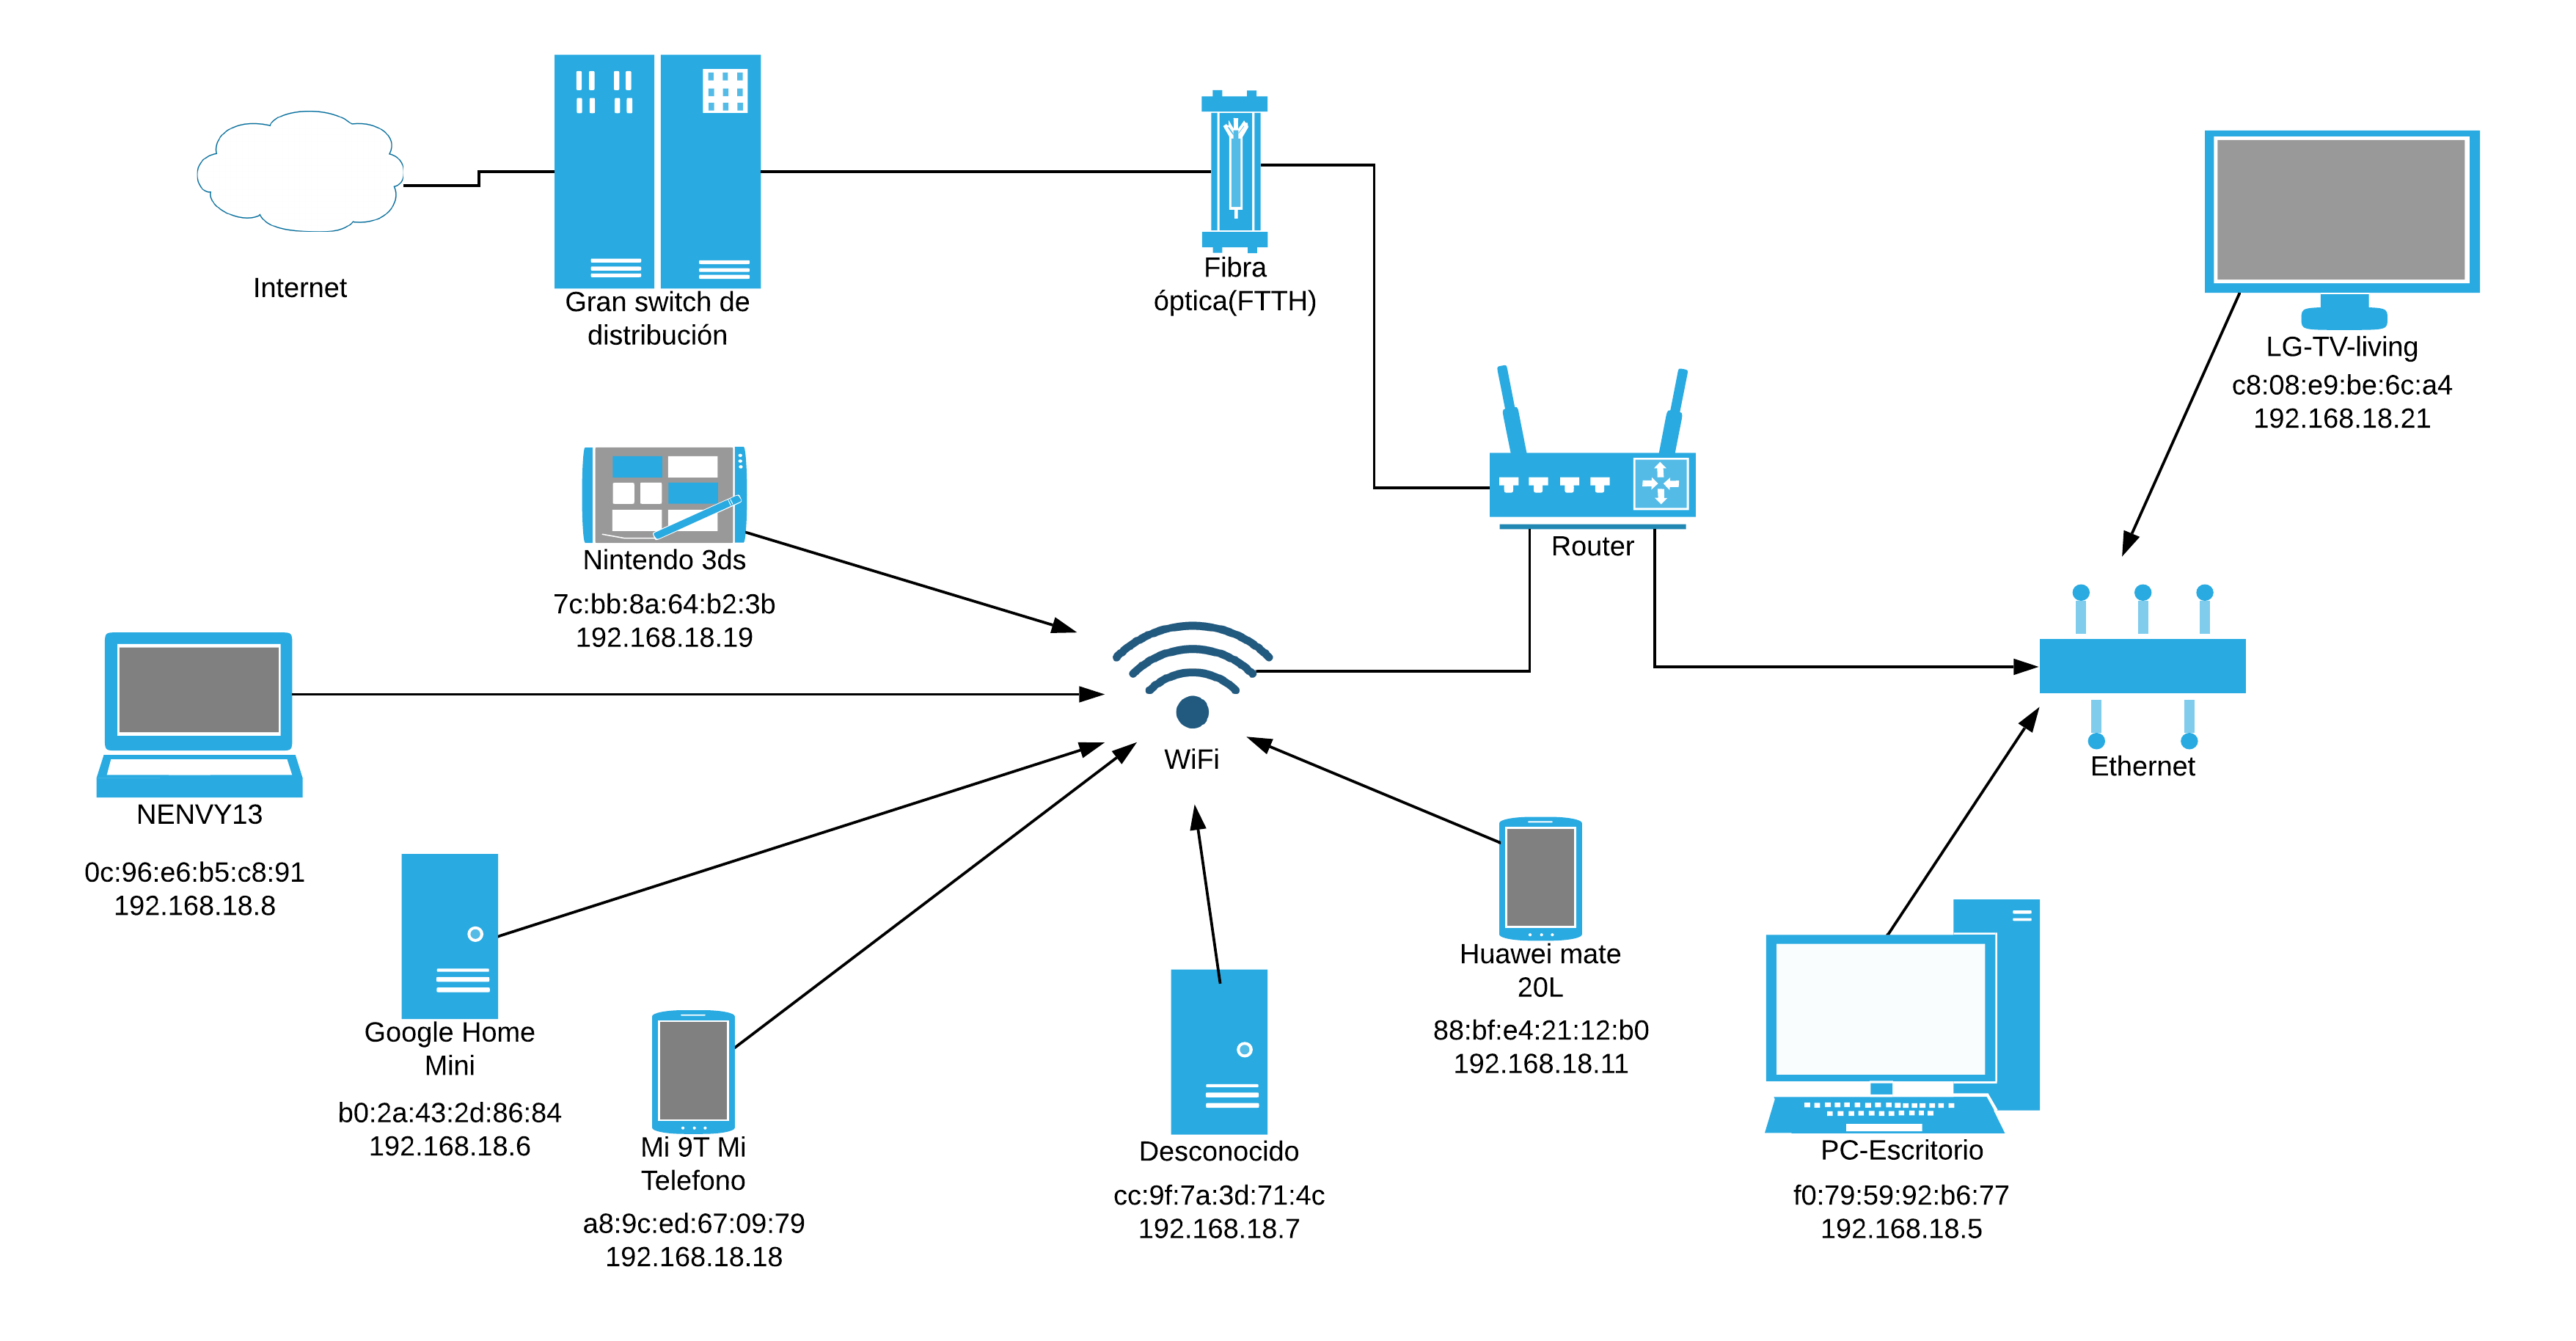
\includegraphics[scale=0.57]{images/Diagrama de Red (1).png}
	\caption{Diagrama de red con los dispositivos conectados al momento de hacer el análisis }
	\label{diag:red}
\end{figure}


\noindent Conociendo la red y las ips de los dispositivos se procede a hacer un análisis de la velocidad de transmisión entre dos dispositivos. Con ayuda de la herramienta \verb|iperf3| se ha creado un servidor en el dispositivo \textbf{PC-Escritorio} con la ip local \verb|192.168.18.5| . Cabe destacar que este dispositivo posee un sistema operativo Windows 10 el cual posee un subsistema de Linux en el cual se puede instalar \verb|iperf3|. Teniendo esto en cuenta en el dispositivo \textbf{PC-Escritorio} se establece el comando :

\begin{lstlisting}
$ iperf3 -s
\end{lstlisting}

\noindent Ahora en el dispositivo \textbf{NENVY13} con la ip local \verb|192.168.18.8| el cual está conectado al Wifi con 5G, se ejecuta el siguiente comando:

\begin{lstlisting}
$ iperf3 -c 192.168.18.5 -u -b XM
\end{lstlisting}



\noindent Donde X toma valores entre 1 a 1000, los cuales representan el ancho de banda en Megabits. Para esta sección se han hecho diferentes pruebas, modificando X, los cuales tomaron valores [1,10,100,200,300,400,500,1000] de lo que se obtuvo el siguiente gráfico:

\begin{figure}[!h]
	\centering
	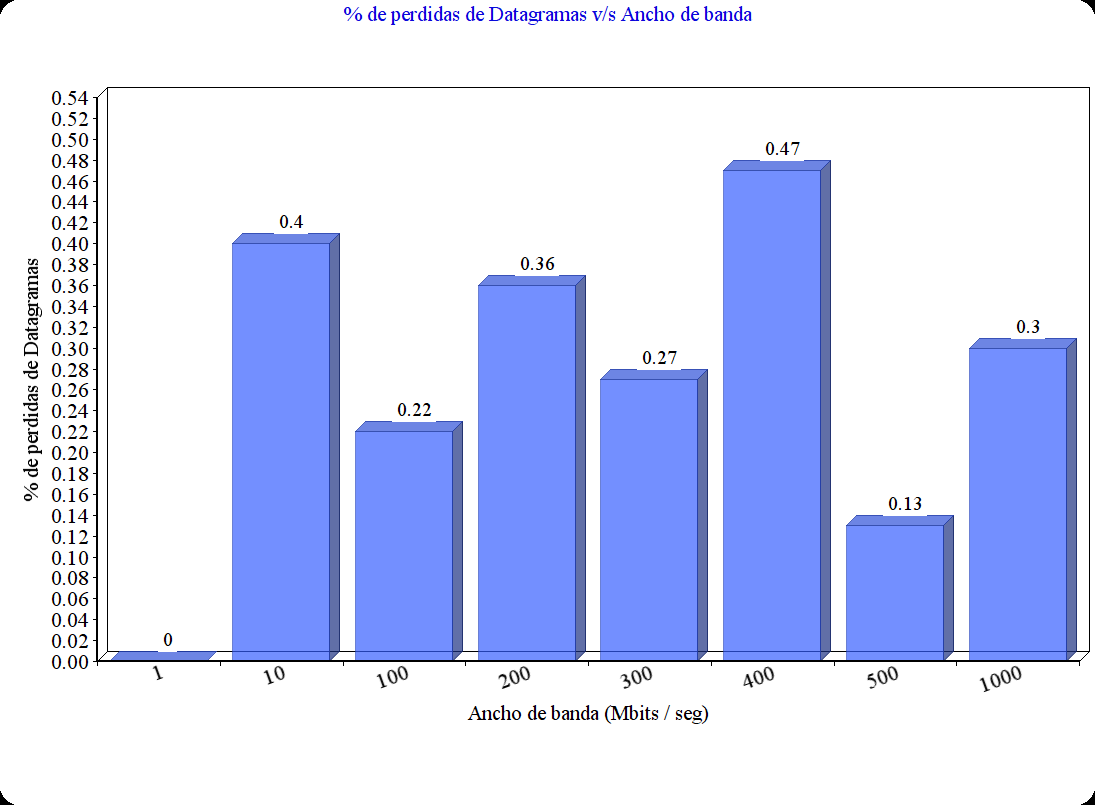
\includegraphics[scale=0.5]{images/graph.png}
	\caption{Gráfico del \% de datagramas perdidos v/s Ancho de banda en 5G}
	\label{diag:iperf3}
\end{figure}



\subsection{Protocolo ARP}
 
 \noindent En esta sección se estudiará el protocolo ARP mediante \verb|Wireshark|. En el Marco Teórico se puede encontrar más información sobre Wireshark y el protocolo ARP. 
 
 
 \subsubsection{Capturando paquetes con Wireshark}
 
 Primeramente, para empezar a capturar datos con Wireshark, se ha instalado la herramienta con el siguiente comando: 
 
 \begin{lstlisting}
$ sudo apt install libcap2-bin wireshark
\end{lstlisting}

\noindent Luego para comenzar a capturar paquetes con esta herramienta se utiliza el siguiente comando: 
 \begin{lstlisting}
$ sudo wireshark 
\end{lstlisting}

Al iniciar se debe colocar la interfaz de red que se está utilizando, en el caso particular de esta experiencia es \verb|wlo1|.

\noindent Es importante iniciarlo en modo súper usuario debido a que Wireshark necesita permisos para capturar todos los paquetes de la red. Luego, cuando ya se ha iniciado el programa,se comienza de inmediato la captura de paquetes que circulan por la red a los diferentes dispositivos.

\begin{figure}[!ht]
	\centering
	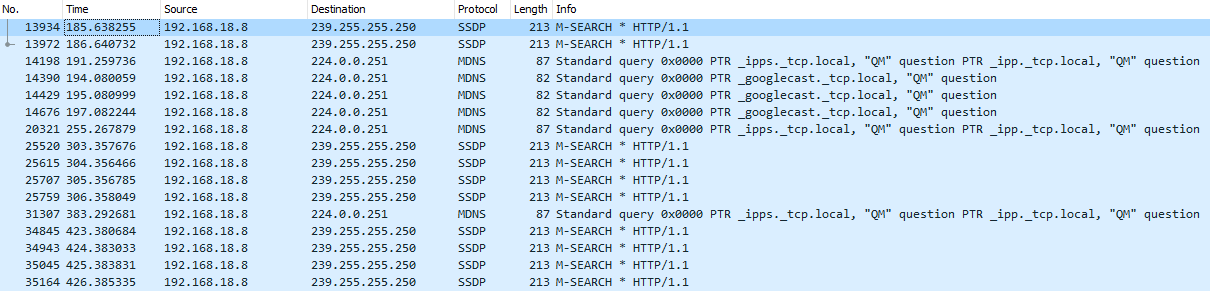
\includegraphics[scale=0.5]{images/wireshark1.png}
	\caption{Imagen de Wireshark capturando datos de los dispositivos conectados}
	\label{fig:wire1}
\end{figure}


\noindent Como se puede ver en la figura \ref{fig:wire1} Wireshark proporciona información sobre el origen y destino de la data que está circulando, aparte del protocolo utilizado. Lo interesante de esta aplicación es que se puede filtrar por ips y saber con qué ip se está comunicando cierto dispositivo. Por ejemplo, si se fija la ip de destino del \textbf{PC-Escritorio} (\verb|192.168.18.5|). Para fijar un filtro, en la parte superior de la tabla de datos, se puede colocar \verb|ip.dst == 192.168.18.5| lo cual da: 

\begin{figure}[!ht]
	\centering
	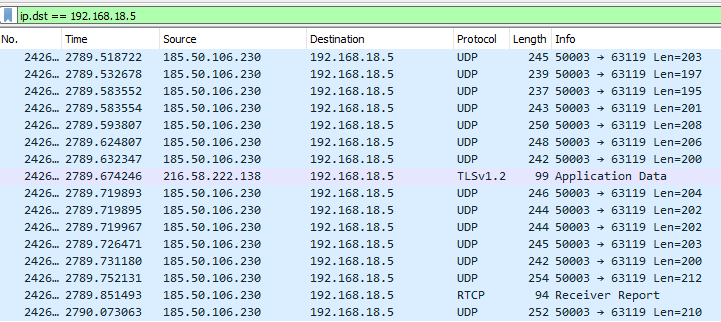
\includegraphics[scale=0.6]{images/wireshark2.png}
	\caption{Imagen de Wireshark con filtro de ip de destino}
	\label{fig:wire2}
\end{figure}


\subsubsection{Obteniendo información de las tablas ARP}

\noindent Como se veia en el capítulo de marco teórico, el protocolo ARP posee tablas almacenadas en caché que guardan datos de las direcciones físicas de los dispositivos de la red asociadas a una ip local. Es por eso que ahora se estudiará que datos se almacenan en el dispositivo de prueba \textbf{NENVY13} (\verb|192.168.18.8|).
\newline

\noindent Entonces antes de comenzar a obtener la tabla ARP actual, se partirá desde un comienzo con la tabla vacía. Para vaciar la tabla se ha utilizado el siguiente comando: 

 \begin{lstlisting}
$ sudo ip -s -s neigh flush all
\end{lstlisting}

\noindent Como ya se ha vaciado la tabla ARP del dispositivo, se puede obtener la tabla actual con el comando:

 \begin{lstlisting}
$ arp -n
\end{lstlisting}
 
 \noindent En el comando anterior, no existe mayor diferencia si se ejecuta en modo súper usuario o no. Entonces al ejecutar el código anterior se obtiene:
 
 \begin{figure}[!ht]
	\centering
	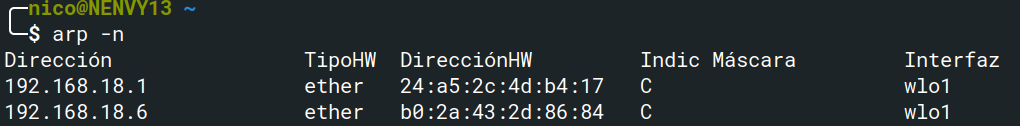
\includegraphics[scale=0.4]{images/arp_1.png}
	\caption{Imagen resultado de la tabla ARP luego de vaciarla}
	\label{fig:arp1}
\end{figure}
 
 \noindent Ahora para probar si la tabla se actualiza correctamente, se ha hecho \verb|$ ping 192.168.18.8| de los siguientes dispositivos:
 
 \begin{enumerate}
     \item PC-Escritorio (\verb|192.168.18.5|)
     \item Mi9T-MiTelefono (\verb|192.168.18.18|)
 \end{enumerate}
 
 \noindent Ahora se ha vuelto a ver la tabla ARP del dispositivo con el comando antes mencionado:
 
 \newpage
 
\begin{figure}[!ht]
	\centering
	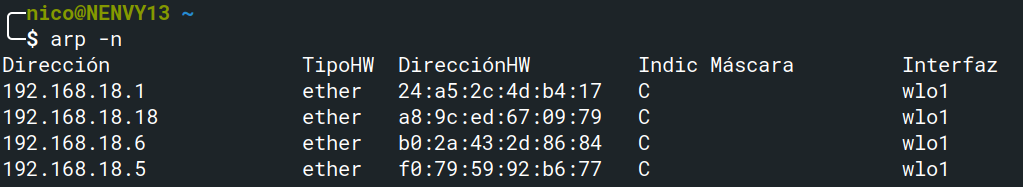
\includegraphics[scale=0.4]{images/arp_2.png}
	\caption{Imagen de la nueva tabla ARP después de hacer pings}
	\label{fig:arp2}
\end{figure}

\noindent Lo que continua en la siguiente sección se analizará que ocurre en Wireshark mientras se hace el ping al dispositivo.
